\documentclass[final,dvipsnames]{beamer}



\PassOptionsToPackage{english}{babel}
\PassOptionsToPackage{
  size = custom,
  width = 80,
  height = 110,
  scale = 1.5,
  debug,
}{beamerposter}


\usepackage{utfprpgtex-poster}
\usepackage{graphicx}
\usepackage[absolute,overlay]{textpos}
\usepackage{color}
\usepackage{tikz}
\usetikzlibrary{shadings}
\usepackage{amsmath,amssymb,latexsym}
\usepackage[many]{tcolorbox}

\newtcolorbox{subblock}[1][]{
  beamer,
  no shadow,
  width=\textwidth+7pt,
  enlarge left by=-3pt,
  colframe=block body.bg,
  bottom=0pt,
  top=0pt,
  left=0pt,
  right=0pt,
  boxrule=0cm,
  toptitle=0pt,
  bottomtitle=-1pt,
  fonttitle=\normalfont,
  adjusted title=#1,
  interior titled code={
    \shade[left color=Maroon!80,right color=Dandelion,middle color=Salmon] 
      (title.south west) --
      (title.south east) {[rounded corners] -- 
      (title.north east)  -- 
      (title.north west)} --
      (title.south west); 
  }
}


\title{
  Automatic Driving
}

\author{
  DeeCamp Team 40 - Racer Zero
}

\date{}

%% ----- Contents -----
\begin{document}

\begin{frame}[t, fragile = singleslide]{}

\begin{columns}[t]

\begin{column}{0.02\textwidth}
\end{column}

%% Logo
\begin{column}{0.16\textwidth}
\flushleft

\includegraphics[width = 0.8\columnwidth]{./assets/deecamp_logo.jpg}
\end{column}

%% ----- Title -----
\begin{column}{0.6\textwidth}
\titlepage
\end{column}

\begin{column}{0.24\textwidth}
\end{column}

\end{columns}

%% ----- Content -----
\begin{columns}[t]

%% ----- Column 1 -----
\begin{column}{0.3\textwidth}

%% Task Overview
\begin{block}{Task Overview}
  \begin{itemize}
    \item Our task is to deploy an end-to-end automatic driving system on a real car, including perception, model inference and control submodules.
  \end{itemize}
  %% Car photo
  \begin{figure}[ht]
    \centering
    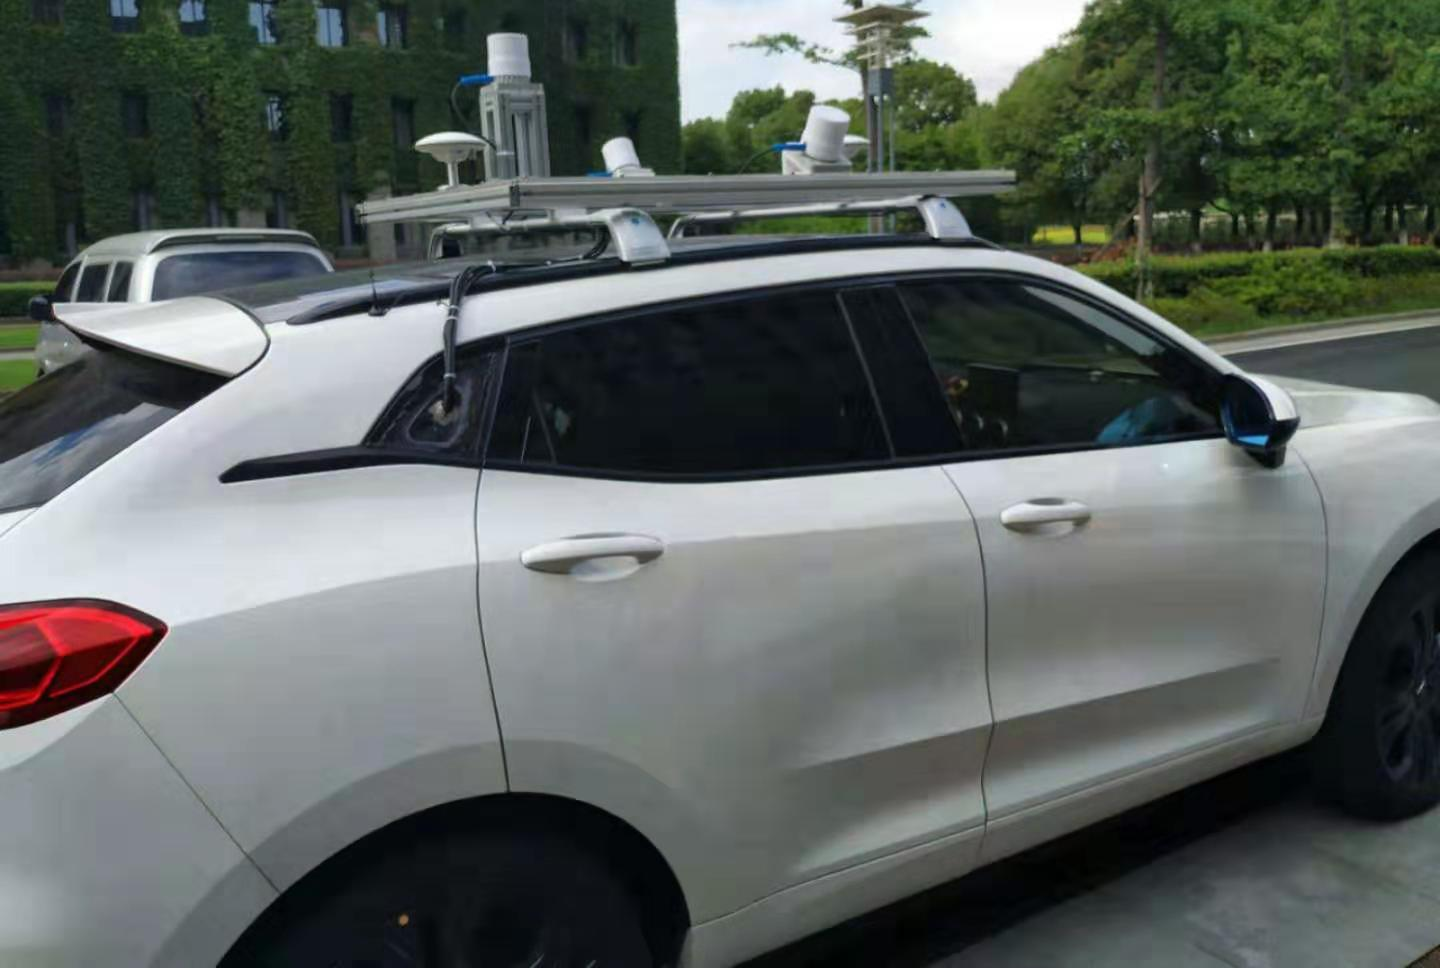
\includegraphics[width = 0.6\columnwidth]{./assets/auto_car.jpeg}
    \caption{Our Automatic Driving Car}
    \label{fig:label}
  \end{figure}

  %% System
  \begin{figure}[ht]
    \centering
    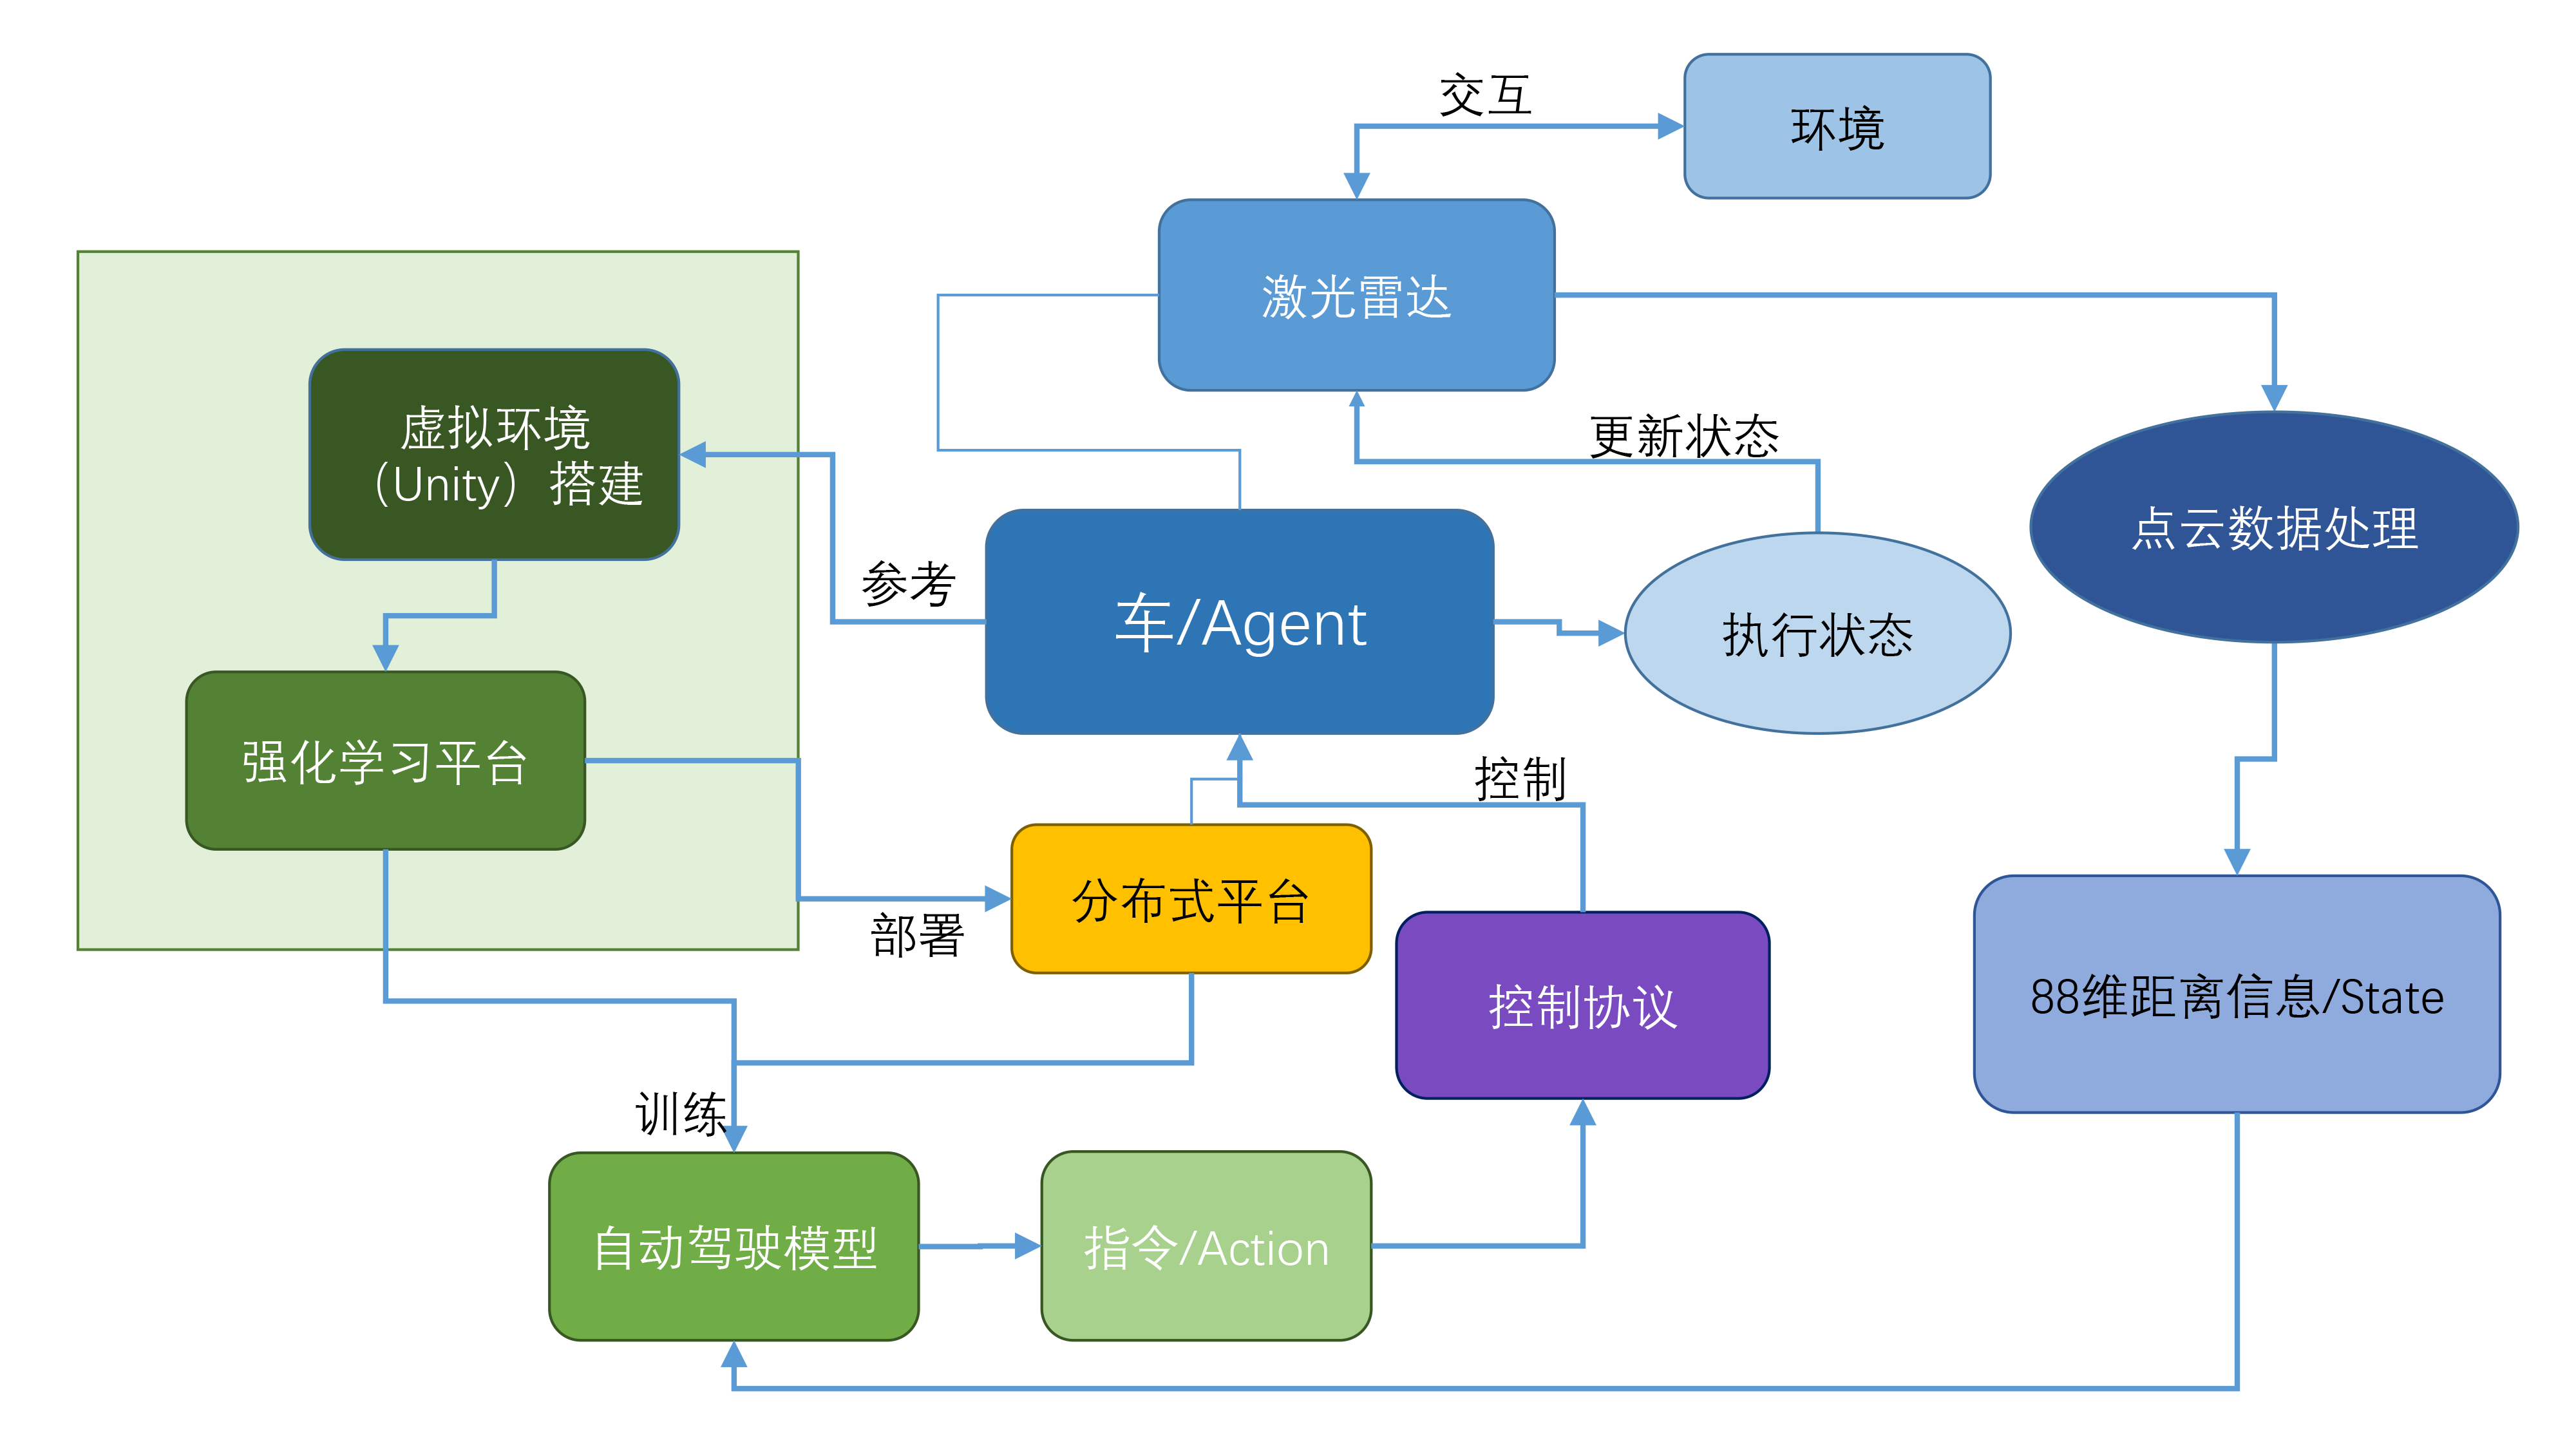
\includegraphics[width = \columnwidth]{./assets/system.jpeg}
    \caption{Our System Architecture}
    \label{fig:label}
  \end{figure}
\end{block}

%% Contribution
\begin{block}{Contribution}
  \begin{itemize}
    \item Design a reinforcement learning algorithm with PPO.
    \item Design a LIDAR perception data fusion algorithm.
    \item Model integration \& interface deployment.
  \end{itemize}
\end{block}

%% Approach
\begin{block}{Approach}

%% Training environment
  \begin{subblock}[Training Environment]
  \begin{itemize}
    \item We employ 8 high performance machines, each with 2 NVidia 2080Ti GPU.
    \item Ray \& RLlib: We use scalable and distributed reinforcement learning lib to accelerate training process.
  \end{itemize}
  \begin{figure}[ht]
    \centering
    
\includegraphics[width = 0.6\columnwidth]{./assets/ray_logo.png}
    \caption{Ray Lib}
    \label{fig:label}
  \end{figure}
  \end{subblock}

%% LIDAR Algorithm
  \begin{subblock}[LIDAR Algorithm]
  \begin{itemize}
    \item There is a blind area near the LIDAR.
    \item With 3 LIDAR, we design a data fusion and context perception algorithm to shrink blind area.
  \end{itemize}
  \end{subblock}

\end{block}
\end{column}

%% ----- Column 2 -----
%% RL Algorithm
\begin{column}{0.3\textwidth}
\begin{subblock}[RL Algorithm]
  \begin{itemize}
    \item We train our model in a simulator powered by ml-agents.
    \begin{figure}[ht]
    \centering
    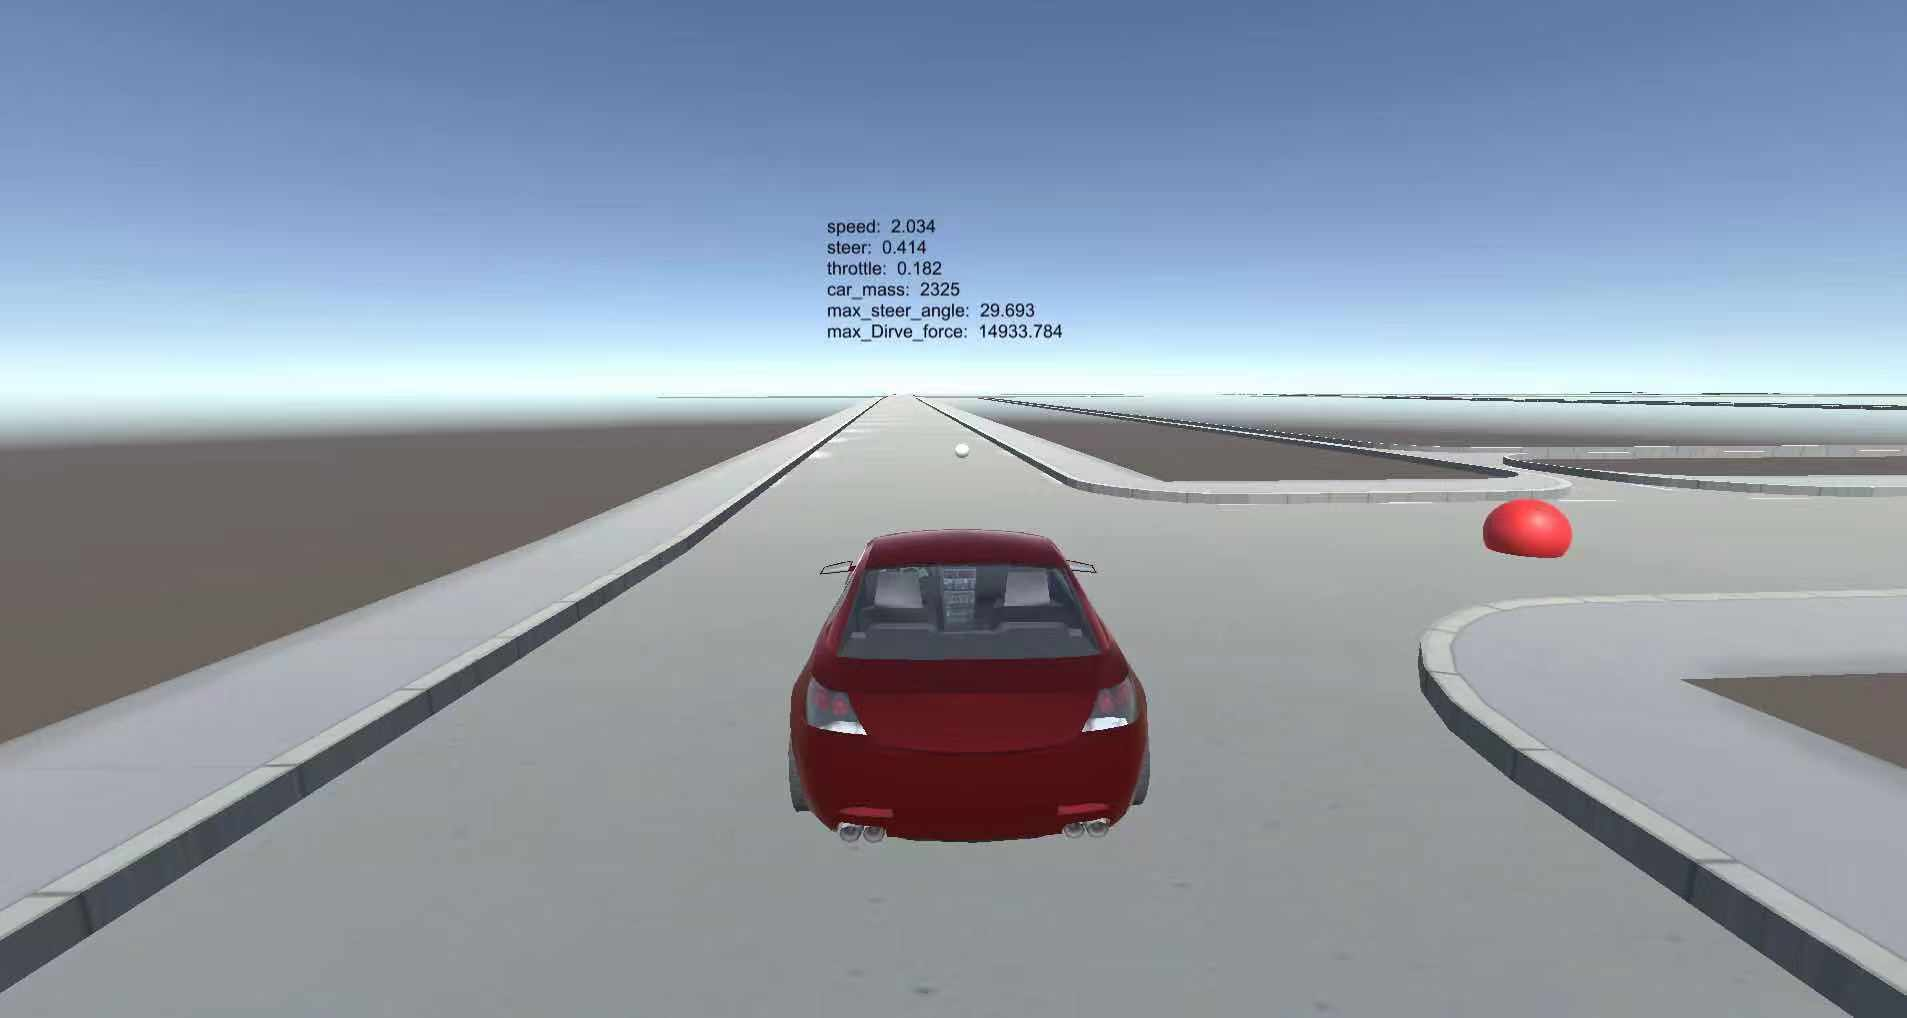
\includegraphics[width = 0.9\columnwidth]{./assets/simulator.jpeg}
    \caption{Simulator}
    \label{fig:label}
  \end{figure}
  \end{itemize}
\end{subblock}

%% CAN Interface
\begin{subblock}[CAN Interface]
  
\end{subblock}
\end{column}

%% ----- Column 3 -----
\begin{column}{0.3\textwidth}

%% Experiment Results
\begin{block}{Experiment Results}

\end{block}

%% Conclusion
\begin{block}{Conclusion}

\end{block}

%% Reference
\begin{block}{Reference}

\end{block}
\end{column}

\end{columns}
\end{frame}
\end{document}